\def\probtitle{불꽃놀이의 아름다움 2}
\def\probno{G} % 문제 번호

\begin{problem}{\probno{}. \probtitle{}}

봄 축제 때 정보과학관에서는 아무 행사도 진행되지 않는다는 것에 화가 난 민성이는 정보과학관 입구 앞에서 직접 불꽃놀이 행사를 진행하려고 한다.

민성이는 정보과학관 입구 앞에 $N$개의 폭죽과 서로 다른 두 폭죽을 직접 연결하는 도화선 $N$개를 설치했다. $N$개의 폭죽은 도화선을 통해 모두 직간접적으로 연결되어 있다. 즉, 어떤 한 폭죽에 불을 붙이면 도화선을 따라 모든 $N$개의 폭죽에 불이 붙는다.

민성이는 도화선으로 직접 연결된 두 폭죽의 색이 다를 때 불꽃놀이가 아름답다고 생각한다. 하지만 불꽃놀이의 색의 종류를 늘리는 것은 비용이 많이 들기 때문에 최소 개수의 색을 사용하려고 한다. 아름다운 불꽃놀이를 만들기 위해 필요한 색의 개수의 최솟값을 구해보자.


\InputFile

첫째 줄에 폭죽의 개수 $N$이 주어진다.

둘째 줄부터 $N$개의 줄에 걸쳐, $i$번째 도화선이 연결하는 두 폭죽의 번호 $a_i,b_i$가 공백으로 구분되어 주어진다.

\OutputFile

아름다운 불꽃놀이를 만들기 위해 필요한 폭죽 색 종류의 최솟값을 출력한다.

\Constraints

\begin{itemize}[topsep=0pt,noitemsep]
    \item $3\leq N\leq 200\,000$ 
    \item $1\leq a_i,b_i\leq N$ ($1 \le i \le N$)
    \item $N$개의 폭죽은 도화선을 통해 모두 서로 연결되어 있다.
    \item 도화선은 서로 다른 두 폭죽을 연결하며, 다른 도화선이 같은 쌍을 연결하는 경우는 없다. 
    \item 입력으로 주어지는 수는 모두 정수이다.
\end{itemize}

\Example

\begin{example}
    \exmpfile{./example/01.in.txt}{./example/01.out.txt}%
    \exmpfile{./example/02.in.txt}{./example/02.out.txt}%
\end{example}

\Notes
\usetikzlibrary{patterns}
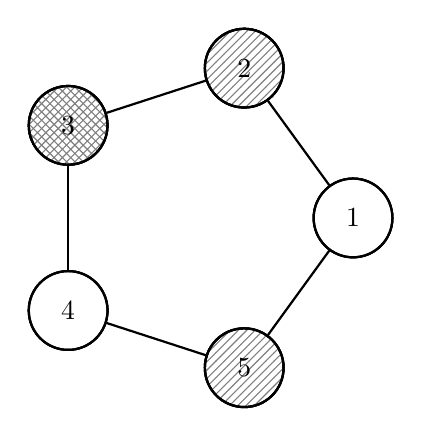
\begin{tikzpicture}[scale=2, every node/.style={circle, draw, thick, minimum size=1cm}]

\tikzset{
    color1/.style={fill=white},
    color2/.style={pattern=north east lines, pattern color=gray},
    color3/.style={pattern=crosshatch, pattern color=gray}
}

\foreach \i in {1,...,5} {
    \node[thick] (v\i) at ({72 * (\i - 1)}:1) {};
}

\foreach \i in {1,...,5} {
    \pgfmathtruncatemacro{\nexti}{mod(\i, 5) + 1}
    \draw[thick] (v\i) -- (v\nexti);
}

\node[color1] at (v1.center) {};
\node[color2] at (v2.center) {};
\node[color3] at (v3.center) {};
\node[color1] at (v4.center) {};
\node[color2] at (v5.center) {};

\foreach \i in {1,...,5} {
    \node at (v\i) {\i};
}

\end{tikzpicture}

첫 번째 예시는 위 그림과 같이 3개의 색을 이용하면 아름다운 불꽃놀이를 만들 수 있고, 이보다 더 적은 색으로는 만들 수 없다.

\end{problem}